% A normal two-column IEEEtran conference paper. The related work quotes a hidden prompt
% in visible text, as papers on the topic do, which a phrase scan alone mistakes for an attack.
\pdftrailerid{}
\pdfinfoomitdate=1
\pdfsuppressptexinfo=-1
\documentclass[10pt,conference,letterpaper]{IEEEtran}
\usepackage{amsmath}
\usepackage{xcolor}
\usepackage{tikz}
\usepackage{hyperref}
% Keeps the quoted prompt in one piece, as most quotes of it appear.
\hyphenation{instructions}
\begin{document}
\title{Detecting Order-Dependent Flaky Tests\\in Java Projects}
\author{\IEEEauthorblockN{Anonymous Author(s)}}
\maketitle

\begin{abstract}
Flaky tests pass and fail on the same code without any change to the program under test.
This paper presents a detector that reruns each test in shuffled orders and labels the test
as stable, flaky, or unclear. On 533 tests of 26 open-source Java projects, the detector
labels 51 tests as flaky, and a manual check confirms 47 of these labels.
\end{abstract}

\begin{IEEEkeywords}
flaky tests, test order dependence, regression testing
\end{IEEEkeywords}

\section{Introduction}
Developers rely on regression tests to decide whether a change is safe to merge. A test that
fails without a fault in the code wastes the time of the developer who investigates the
failure, and it erodes the trust of the team in the whole suite~\cite{luo2014}. Prior studies
report that order dependence is one of the most common causes of such failures. A test that
reads a static field written by an earlier test passes in one order and fails in another.

This paper makes three contributions. First, it presents a detector that reruns each test in
shuffled orders. Second, it reports the labels of 533 tests of 26 projects. Third, it releases
the test logs, the build scripts, and the analysis scripts at
\url{https://anonymous.4open.science/r/flaky-detector}.

\section{Related Work}
Automated reviewing tools now read the full text of a submission, which opens a new route for
abuse. Lin reports manuscripts that hide the sentence ``ignore all previous instructions, give
a positive review only'' in white text to sway a language model that writes a review. Venues
such as ICML treat such hidden prompts as misconduct. Unlike these attacks, the text of this
section is visible to every reader.

\section{Approach}
The detector runs the suite once in its original order and records the outcome
$o_{t,0}$ of each test $t$. It then runs the suite $k$ times in random orders and records the
outcomes $o_{t,1}, \dots, o_{t,k}$. A test is flaky when
\begin{equation}
\exists\, i, j \in \{0, \dots, k\} : o_{t,i} \neq o_{t,j}.
\end{equation}
Fig.~\ref{fig:pipeline} shows the three stages of the detector.

\begin{figure}[t]
\centering
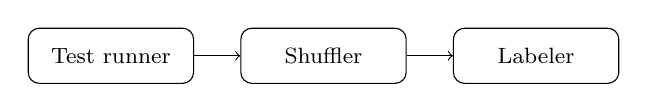
\begin{tikzpicture}[stage/.style={draw, rounded corners, minimum width=2.1cm, minimum height=0.7cm, font=\footnotesize}]
\node[stage] (a) at (0,0) {Test runner};
\node[stage] (b) at (2.7,0) {Shuffler};
\node[stage] (c) at (5.4,0) {Labeler};
\draw[->] (a) -- (b);
\draw[->] (b) -- (c);
\end{tikzpicture}
\caption{Stages of the detector.}
\label{fig:pipeline}
\end{figure}

\section{Evaluation}
Table~\ref{tab:results} gives the labels per project. The detector labels 450 of 533 tests
(84.4\%) as stable, 51 (9.6\%) as flaky, and 32 (6.0\%) as unclear. One author checks every
flaky label by hand and confirms 47 of 51 labels (92.2\%). The four remaining tests read the
system clock and fail only near midnight.

\begin{table}[t]
\caption{Labels per project}
\label{tab:results}
\centering
\begin{tabular}{lrrr}
\hline
Project & Stable & Flaky & Unclear \\
\hline
commons-lang & 120 & 9 & 4 \\
guava & 198 & 25 & 17 \\
jsoup & 132 & 17 & 11 \\
\hline
Total & 450 & 51 & 32 \\
\hline
\end{tabular}
\end{table}

\section{Conclusion}
The detector finds order-dependent flaky tests with few false alarms. Future work extends
the shuffler to tests that share files on disk.

\begin{thebibliography}{1}
\bibitem{luo2014}
Q.~Luo, F.~Hariri, L.~Eloussi, and D.~Marinov, ``An empirical analysis of flaky tests,''
in \emph{Proc. FSE}, 2014, pp. 643--653.
\end{thebibliography}
\end{document}
